% !TeX root = Proposal.tex

% =========================================================================
%
% This proposal will be written as an article
%
% =========================================================================
\documentclass[11pt,a4paper,titlepage]{article}

%opening
\title{PhD Research Proposal}
\author{Harold Ship \\ University of Haifa}
% =========================================================================
%
% This part of the preamble is the package importing and setup
%
% =========================================================================


% UTF file input
\usepackage[utf8]{inputenc}
\usepackage[T1]{fontenc}
\usepackage[english]{babel}

% math stuff
\usepackage{amsmath}
\usepackage{amsfonts} % for mathbb
\usepackage{mathtools} % loads amsmath plus other tools
\usepackage{fixmath} % fix greek letters
\usepackage{relsize} % for \mathlarger
\usepackage{bm}

% math theorems and theorem environments
\usepackage{amsthm}

% biblatex for references
\usepackage{csquotes} % ensures biblatex quotes things correctly
\usepackage[backend=biber,style=apa,autocite=inline]{biblatex}
\DeclareLanguageMapping{english}{english-apa}
\addbibresource{../personal_bibliography.bib}

% puts hyperlinks in PDF. Must be loaded before cleveref
\usepackage{hyperref}
\hypersetup{hypertexnames=false}

% better cross-refs like Equations, etc
\usepackage{cleveref}

% Glossary, acronym
\usepackage[acronym,toc,nonumberlist]{glossaries}
\makeglossaries

% drawings
\usepackage{tikz}
\usetikzlibrary{positioning}% To get more advances positioning options
\usetikzlibrary{arrows}% To get more arrow heads
\tikzset{compartment/.style={%
        rectangle,
        rounded corners=9pt,
        text height=0.75cm,
        text depth=.5cm,
        text width=1cm,
        text centered,
        draw=black!50,
        fill=black!20
    }}

% =========================================================================
%
% My macros
%
% =========================================================================
\renewcommand*{\vec}[1]{\ensuremath{\bm{#1}}}%
\newcommand*{\mat}[1]{\ensuremath{\mathrm{#1}}}%
\newcommand*{\transpose}[1]{\ensuremath{#1^{\mathrm{T}}}}%
\newcommand*{\dd}{\ensuremath{\mathop{}\!\mathrm{d}}}%
\newcommand*{\dt}[1]{\ensuremath{#1^{\prime}}}%
\newcommand*{\R}{\ensuremath{\mathop{}\!\mathbb{R}}}%
\newcommand*{\RR}[1]{\ensuremath{\mathop{}\!\mathbb{R}^{#1}}}%
\newcommand*{\optimal}[1]{\ensuremath{#1^*}}%
\newcommand*{\uncertainset}[1]{\ensuremath{\mathcal{#1}}}%
\newcommand*{\defnterm}[1]{\textbf{#1}}%

% math theorem environments (must be after cleveref)
\theoremstyle{definition}
\newtheorem{assumption}{Assumption}
\newcommand{\assumptionautorefname}{Assumption}

\begin{document}

\pagenumbering{roman}

% =========================================================================
% Make the title page and other boilerplate
% =========================================================================
\maketitle \clearpage
\tableofcontents \clearpage
\iffalse % remove to enable list of figures and tables
\listoffigures \clearpage
\listoftables \clearpage
\fi
\printglossary[type=\acronymtype] \clearpage


\pagenumbering{arabic}
\setcounter{page}{1}

%\begin{abstract}
%
%\end{abstract}

% =========================================================================
% Mathematical and Statistical Models
% =========================================================================
\section{Mathematical Models}
\label{sec:math-models}

\subsection{SIR Model}
\label{subsec:math-models:sir}

The SIR model is a \textbf{compartmental model},
meaning that the population is divided into distinct groups \autocite{keeling2011modeling}.
Over time,
the size of the group can change.
For SIR,
these groups are:

\begin{tabular}{cl}
    $S$ & the \textbf{susceptible} group,%
    who can acquire the disease\\%
    $I$ & the \textbf{infectious} group,%
    who have the disease and can infect others\\%
    $R$ & the \textbf{recovered} group,%
    who are no longer infectious nor susceptible
\end{tabular}

Individuals can go from $S$ to $I$ and from $I$ to $R$,
as indicated in \autoref{fig:compartment-flow-sir}.

\begin{figure}
    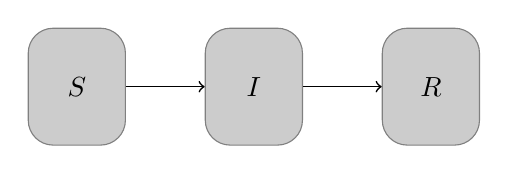
\begin{tikzpicture}
        \node [compartment] (S) at (0,0) {$S$};
        \node [compartment] (I) [right=of S]  {$I$};
        \node [compartment] (R) [right=of I]  {$R$};
        \path[semithick,->] (S) edge node {} (I);
        \path[semithick,->] (I) edge node {} (R);
    \end{tikzpicture}
    \caption{
        \label{fig:compartment-flow-sir}
        Susceptible individuals can become infected.
        Infected can recover.
    }
\end{figure}

We have $S + I + R = N$ where $N$ is the population size.
If we assume that $N$ does not change over time,
then without loss of generality we can assume $N=1$ in order to simplify the model.

\begin{align}
    \dt{S} & =  - \beta S I \\%
    \dt{I} & = \beta S I - \gamma I \\%
    \dt{R} & = \gamma I%
\end{align}

The model above requires the following parameters,
or \textit{data}:

\begin{tabular}{cl}
    $\beta$ & product of the contact rates and transmission probability\\%
    $\gamma$ & recovery rate
\end{tabular}

Note that $1/\gamma$ is the \textit{average infectious period}.

\subsection{SEIR Model}
\label{subsec:math-models:seir}

The SEIR model builds on the SIR model described in \autoref{subsec:math-models:sir} by adding an additional compartment $E$,
which contains members of the population who have been acquired the disease,
but the disease is latent in them;
that is,
it is in some sort of incubation period.
They are not yet infectious.
The progression from compartment to compartment is shown in \autoref{fig:compartment-flow-seir}.

\begin{figure}
    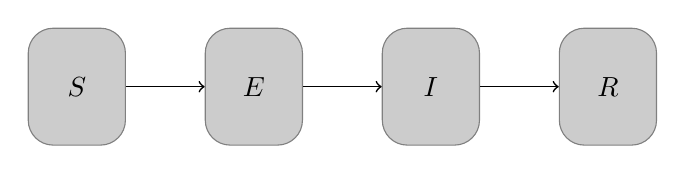
\begin{tikzpicture}
    \node [compartment] (S) at (0,0) {$S$};
    \node [compartment] (E) [right=of S]  {$E$};
    \node [compartment] (I) [right=of E]  {$I$};
    \node [compartment] (R) [right=of I]  {$R$};
    \path[semithick,->] (S) edge node {} (E);
    \path[semithick,->] (E) edge node {} (I);
    \path[semithick,->] (I) edge node {} (R);
    \end{tikzpicture}
    \caption{
        \label{fig:compartment-flow-seir}
        Susceptible individuals can become exposed.
        Exposed then become infected.
        Infected can recover.
    }
\end{figure}

We have $S + E + I + R = N$ where $N$ is the population size.
If we assume that $N$ does not change over time,
then without loss of generality we can assume $N=1$ in order to simplify the model.

\begin{align}
    \dt{S} & = \mu - (\beta I + \mu) S \\%
    \dt{E} & = \beta S I - (\mu + \sigma) E \\%
    \dt{I} & = \sigma E - (\mu + \gamma) I \\%
    \dt{R} & = \gamma I - \mu R %
\end{align}

The parameters or data of the SEIR model is:

The model above requires the following parameters,
or \textit{data}:

\begin{tabular}{cl}
    $\beta$ & product of the contact rates and transmission probability\\%
    $\gamma$ & recovery rate \\%
    $\sigma$ & latent-to-infectious rate
\end{tabular}

\subsection{Age of Infection Model}
\label{subsec:math-models:aoi}

Age of Infection is a discrete time compartmental model.

\subsubsection{Math Model}

\begin{align}
    i(t) \sim \operatorname{Poisson} \left( R(t) \frac{S(t-1)}{N} \sum\limits_{\tau=1}^{T_G} {P_G(\tau)i(t-\tau)} \right) & \\
    S(t) = S(t - 1) - i(t), ~t=1,\ldots,T &
\end{align}

\begin{tabular}{ll}
    $N$ & population size \\
    $i(t)$ &  number of newly infected on day $t$ \\
    Once infected, infectious for $d$ days
    $i(t-\tau)$ & the number of infective people with age-of-infection $\tau$ on day $t$ \\
    $P_{\tau}$ & the probability that infective person with age-of-infection $\tau$ infects a susceptible that they meet \\
    $\beta$ & number of contacts per day \\
    $S(t)$ &  is the number of susceptible individuals on day $t$ \\
    $N$ & is the population size \\
    $P_G$ & the generation-time distribution \\
    $R(t)$ &  the reproductive number on day $t$ \\
\end{tabular}

The initial conditions for the model are $i(0)$ (a vector of length $T_G$) and $S(0)$ (a scalar)

\subsubsection{Observation Model}

\begin{equation}
    Y(t) \sim \operatorname { Poisson }\left(p_{Y} \sum_{\tau=1}^{T_{Y}} P_{Y}(\tau) i(t-\tau)\right)
\end{equation}

\begin{tabular}{ll}
    $Y(t)$ & the number of **newly **observed cases on day $t$ (confirmed / hospitalized / dead). \\
    $i(t)$ & the number of newly infected individuals on day $t$ given by the epidemic model. \\
    $p_Y$ & the probability of an infected case to be observed as $Y$ (detection rate / hospitalization rate / death rate). \\
    $P_Y$ & the time distribution from infection to observation of $Y$ (time to detection / time to hospitalization ...) \\
\end{tabular}

\subsubsection{Identifiability}

The simple case:

\begin{tabular}{ll}
    $i(t) \sim \operatorname{Poisson} \left( R(t) \frac{S(t-1)}{N} \sum\limits_{\tau=1}^{T_G} {P_G(\tau)i(t-\tau)} \right)$ & new cases on day $t$ \\
    $S(t) = S(t - 1) - i(t), ~t=1,\ldots,T$ & susceptible on day $t$ \\
    $Y(t) \sim \operatorname { Poisson }\left(p_{Y} \sum_{\tau=1}^{T_{Y}} P_{Y}(\tau) i(t-\tau)\right)$ & observed cases on day $t$ \\
\end{tabular}

\begin{assumption}
    $i(t)$ above is large enough that it can be approximated by Normal distribution
\end{assumption}
\begin{assumption}
    $P_G(0) = 1, P_G(t) = 0, t > 0$
\end{assumption}
\begin{assumption}
    $p_Y = 1, P_Y(0) = 1$, $P_Y(t) = 0, t > 0$ so that $Y(t) = i(t)$
\end{assumption}
\begin{assumption}
    $S(t-1) \approx N$ that is $S(t-1)/N \approx 1$
\end{assumption}

Then $Y(t) = R(t) i(t-1) + \epsilon_t$ where $\epsilon_t \sim N(0, R(t))$.
The least squares estimate $\hat{R}(t) = \mathop{\mathrm{argmin}}\limits_{R \in \mathcal{R}} \sum\limits_{t=1}^{T} {\left( Y(t) - R(t)i(t-1) \right)^2}$
If $R(t) = \beta$ is constant, then:
$\hat{\beta} = \left(X^{\top} X\right)^{-1}X^{\top} Y$  where:
$X = (i(0), \ldots, i(T-1))^{\top}$,
$Y = (Y(1), \ldots, Y(T))^{\top}$
$\operatorname{Var}(\hat{\beta}) = \frac{\sum{\sigma^2(t)}}{\sum{i(t)^2}}$

So $\beta$ is identifiable if and only if $(X^{\top}X)$ is of full rank.
Next, consider dividing $[0,T]$ into 2 sub-intervals $[0, T^{*}]$ and $[T_{*}, T]$, with

$$
    R(t) =
    \begin{cases}
        \beta_1 & t \in [0,T^{*}] \\
        \beta_2 & t \in [T^{*}, T]
    \end{cases}
$$
where $T^{*}$ is known.
Then $\beta = (\beta_1, \beta_2)$ is identifiable if each of $\beta_1, \beta_2$ are identifiable as above.
More generally, suppose $R(t) = (\beta_1, \ldots, \beta_k), k \ll T$ on intervals $[0, T_1], \ldots, [T_{k-1}, T_k]$. Then $\beta$ is identifiable if each of the $\beta_j$ are identifiable on $[T_{j-1}, T_j]$.
Suppose there is parameter vector $\theta$ such that $R(t) = f(t; \theta)$.



% =========================================================================
% Optimal Control and Interventions
% =========================================================================
\section{Controlling Outbreaks with Interventions}
\label{sec:control}

% =========================================================================
% Causal Inference
% =========================================================================
\section{Causal Inference of Outbreak after Interventions}
\label{sec:causal}




\printbibliography
\label{sec:bibliography}

\end{document}
